\documentclass[a4paper,14pt,oneside,final]{report}

\usepackage[utf8]{inputenc}
\usepackage[russian]{babel}
\usepackage[T2A]{fontenc}
%\usepackage{pscyr}
%\renewcommand{\rmdefault}{cmr}
\usepackage[final,hidelinks]{hyperref}
\usepackage[square,numbers,sort&compress]{natbib}
%\usepackage{times}
\usefont{T2A}{ftm}{m}{sl}
\setlength{\bibsep}{0em}
\PassOptionsToPackage{hyphens}{url}

\usepackage{hyphenat}

\addto\extrasrussian{%
  \def\equationautorefname{формула}%
  \def\figureautorefname{рисунок}%
  \def\listingautorefname{листинг}%
  \def\tableautorefname{таблица}%
}

\addto\captionsrussian{
  \renewcommand\contentsname{\centerline{\bfseries\large{\MakeUppercase{содержание}}}}
  \renewcommand{\bibsection}{\sectioncentered*{Cписок использованных источников}}
  \renewcommand{\listingscaption}{Листинг}
}

\AtEndDocument{

  \addcontentsline{toc}{section}{Cписок использованных источников}%
}
\usepackage{extsizes}


\sloppy

\usepackage{microtype}
\newlength{\fivecharsapprox}
\setlength{\fivecharsapprox}{6ex}


\usepackage{indentfirst}
\setlength{\parindent}{\fivecharsapprox} 

\usepackage[left=3cm,top=2.0cm,right=1.5cm,bottom=2.7cm]{geometry}

\frenchspacing

\usepackage{perpage}
\MakePerPage{footnote}

\makeatletter 
\def\@makefnmark{\hbox{\@textsuperscript{\normalfont\@thefnmark)}}}
\makeatother

\usepackage[bottom]{footmisc}

\makeatletter
\renewcommand{\thesection}{\arabic{section}}
\makeatother

\setcounter{secnumdepth}{3}


% Зачем: Настраивает отступ между таблицей с содержанимем и словом СОДЕРЖАНИЕ
\usepackage{tocloft}
\setlength{\cftbeforetoctitleskip}{-1em}
\setlength{\cftaftertoctitleskip}{1em}


% Зачем: Определяет отступы слева для записей в таблице содержания.
\makeatletter
\renewcommand{\l@section}{\@dottedtocline{1}{0.5em}{1.2em}}
\renewcommand{\l@subsection}{\@dottedtocline{2}{1.7em}{2.0em}}
\makeatother


% Зачем: Работа с колонтитулами
\usepackage{fancyhdr} 
\pagestyle{fancy}


\fancyhf{} 
\fancyfoot[R]{\thepage}
\renewcommand{\footrulewidth}{0pt} 
\renewcommand{\headrulewidth}{0pt}
\fancypagestyle{plain}{ 
    \fancyhf{}
    \rfoot{\thepage}}


% Зачем: Задает стиль заголовков раздела жирным шрифтом, прописными буквами, без точки в конце
\makeatletter
\renewcommand\section{%
  \@startsection {section}{1}%
    {\fivecharsapprox}%
    {-1em \@plus -1ex \@minus -.2ex}%
    {1em \@plus .2ex}%
    {\raggedright\hyphenpenalty=10000\normalfont\bfseries\MakeUppercase}}
\makeatother


% Зачем: Задает стиль заголовков подразделов

\makeatletter
\renewcommand\subsection{
  \@startsection{subsection}{2}
    {\fivecharsapprox}
    {-1em \@plus -1ex \@minus -.2ex}
    {1em \@plus .2ex}
    {\raggedright\hyphenpenalty=10000\normalfont\normalsize\bfseries}}
\makeatother


% Зачем: Задает стиль заголовков пунктов
\makeatletter
\renewcommand\subsubsection{
  \@startsection{subsubsection}{3}%
    {\fivecharsapprox}%
    {-1em \@plus -1ex \@minus -.2ex}%
    {\z@}%
    {\raggedright\hyphenpenalty=10000\normalfont\normalsize\bfseries}}
\makeatother

% Зачем: для оформления введения и заключения, они должны быть выровнены по центру.
\makeatletter
\newcommand\sectioncentered{%
  \clearpage\@startsection {section}{1}%
    {\z@}%
    {-1em \@plus -1ex \@minus -.2ex}%
    {1em \@plus .2ex}%
    {\centering\hyphenpenalty=10000\normalfont\large\bfseries\MakeUppercase}%
    }
\makeatother



% Зачем: Задает стиль библиографии
\bibliographystyle{gost71s2003}

\usepackage[final]{graphicx}
\DeclareGraphicsExtensions{.png,.jpg}

% Зачем: Добавление подписей к рисункам
\usepackage{caption}
\usepackage{subcaption}

% Зачем: поворот ячеек таблиц на 90 градусов
\usepackage{rotating}
\DeclareRobustCommand{\povernut}[1]{\begin{sideways}{#1}\end{sideways}}

\DeclareRobustCommand{\x}[1]{\text{#1}}

% Зачем: Задание подписей, разделителя и нумерации частей рисунков
\DeclareCaptionLabelFormat{stbfigure}{Рисунок \emph{#2}}
\DeclareCaptionLabelFormat{stbtable}{Таблица \emph{#2}}
\DeclareCaptionLabelFormat{stblisting}{Листинг \emph{#2}}
\DeclareCaptionLabelSeparator{stb}{~--~}
\captionsetup{labelsep=stb}
\captionsetup[figure]{labelformat=stbfigure, justification=centering, font={small}}
\captionsetup[listing]{labelformat=stblisting,justification=centering, font={small}}
\captionsetup[table]{labelformat=stbtable,justification=raggedright,  font={small}}
\renewcommand{\thesubfigure}{\asbuk{subfigure}}
% Зачем: Окружения для оформлени<я формул
\usepackage{calc}
\newlength{\lengthWordWhere}
\settowidth{\lengthWordWhere}{где}
\newenvironment{explanation}
    {
    \begin{itemize}[leftmargin=0cm, itemindent=\lengthWordWhere + \labelsep , labelsep=\labelsep]

    \renewcommand\labelitemi{}
    }
    {
    \\[\parsep]
    \end{itemize}
    }


\usepackage{tabularx}

\newenvironment{explanationx}
    {
    \noindent 
    \tabularx{\textwidth}{@{}ll@{ --- } X }
    }
    { 
    \\[\parsep]
    \endtabularx
    }

\usepackage{amsmath}

\usepackage{amsfonts}
\usepackage{amssymb}
\usepackage{amsthm}
\usepackage{calc}
\usepackage{fp}
\usepackage{enumitem}

\makeatletter
 \AddEnumerateCounter{\asbuk}{\@asbuk}{щ)}
\makeatother


\setlist{nolistsep}
\renewcommand{\labelenumi}{\arabic{enumi}.}
\renewcommand{\labelenumii}{\alph{enumii}.}

\setlist[itemize,0]{itemindent=\parindent + 2.2ex,leftmargin=0ex,label=--}
\setlist[enumerate,1]{leftmargin=4em}
%\setlist[enumerate,2]{leftmargin=0em}


% Зачем: Включение номера раздела в номер формулы. Нумерация формул внутри раздела.
\AtBeginDocument{\numberwithin{equation}{section}}

% Зачем: Включение номера раздела в номер таблицы. Нумерация таблиц внутри раздела.
\AtBeginDocument{\numberwithin{table}{section}}

% Зачем: Включение номера раздела в номер рисунка. Нумерация рисунков внутри раздела.
\AtBeginDocument{\numberwithin{figure}{section}}

% Зачем: Включение номера раздела в номер листинга. Нумерация листингов внутри раздела.
\AtBeginDocument{\numberwithin{listing}{section}}


\usepackage{makecell}
\usepackage{multirow}
\usepackage{array}


\usepackage{textcomp}

\usepackage{siunitx}
\sisetup{
  binary-units = true,
  output-decimal-marker = {,},
  per-mode = symbol,
  range-phrase = --,
}
\DeclareSIUnit{\sample}{S}


\newcommand{\ignore}[2]{\hspace{0in}#2}


\usepackage{verbatim}
\usepackage{xcolor}
\usepackage{minted}

%\AtBeginDocument{\numberwithin{lstlisting}{section}}

\usepackage[normalem]{ulem}

\renewcommand{\UrlFont}{\small\rmfamily\tt}

% Магия для подсчета разнообразных объектов в документе
\usepackage{lastpage}
\usepackage{totcount}
\regtotcounter{section}

\usepackage{etoolbox}

\newcounter{totfigures}
\newcounter{tottables}
\newcounter{totreferences}
\newcounter{totequation}

\providecommand\totfig{} 
\providecommand\tottab{}
\providecommand\totref{}
\providecommand\toteq{}

\makeatletter
\AtEndDocument{%
  \addtocounter{totfigures}{\value{figure}}%
  \addtocounter{tottables}{\value{table}}%
  \addtocounter{totequation}{\value{equation}}
  \immediate\write\@mainaux{%
    \string\gdef\string\totfig{\number\value{totfigures}}%
    \string\gdef\string\tottab{\number\value{tottables}}%
    \string\gdef\string\totref{\number\value{totreferences}}%
    \string\gdef\string\toteq{\number\value{totequation}}%
  }%
}
\makeatother

\pretocmd{\section}{\addtocounter{totfigures}{\value{figure}}\setcounter{figure}{0}}{}{}
\pretocmd{\section}{\addtocounter{tottables}{\value{table}}\setcounter{table}{0}}{}{}
\pretocmd{\section}{\addtocounter{totequation}{\value{equation}}\setcounter{equation}{0}}{}{}
\pretocmd{\bibitem}{\addtocounter{totreferences}{1}}{}{}



% Для оформления таблиц не влязящих на 1 страницу
\usepackage{longtable}

\usepackage{gensymb}

% Зачем: преобразовывать текст в верхний регистр командой MakeTextUppercase
\usepackage{textcase}

%  Переносы в словах с тире \hyph.

\def\hyph{-\penalty0\hskip0pt\relax}

% Добавляем левый отступ для библиографии

\makeatletter
\renewenvironment{thebibliography}[1]
     {\sectioncentered*{Cписок использованных источников}
      \@mkboth{\MakeUppercase\refname}{\MakeUppercase\refname}%
      \list{\@biblabel{\@arabic\c@enumiv}}%
           {\settowidth\labelwidth{\@biblabel{#1}}%
            \setlength{\itemindent}{\dimexpr\labelwidth+\labelsep+1em}
            \leftmargin\z@
            \@openbib@code
            \usecounter{enumiv}%
            \let\p@enumiv\@empty
            \renewcommand\theenumiv{\@arabic\c@enumiv}}%
      \sloppy
      \clubpenalty4000
      \@clubpenalty \clubpenalty
      \widowpenalty4000%
      \sfcode`\.\@m}
     {\def\@noitemerr
       {\@latex@warning{Empty `thebibliography' environment}}%
      \endlist}
\makeatother

\newcommand{\intro}[3]{
    \stepcounter{section}
        \sectioncentered*{ПРИЛОЖЕНИЕ \MakeUppercase{#1}}
     \begin{center} 
        \bf{(#2)}\\
        \bf{#3}
    \end{center}
    \markboth{\MakeUppercase{#1}}{}
    \addcontentsline{toc}{section}{Приложение \MakeUppercase{#1} (#2) #3}
}

\begin{document}

\begin{titlepage}
  \begin{center}
    Министерство образования Республики Беларусь\\[1em]
    Учреждение образования\\
    БЕЛОРУССКИЙ ГОСУДАРСТВЕННЫЙ УНИВЕРСИТЕТ \\
    ИНФОРМАТИКИ И РАДИОЭЛЕКТРОНИКИ\\[1em]

    \begin{minipage}{\textwidth}
      \begin{flushleft}
        \begin{tabular}{ l l }
          Факультет & Информационных технологий и управления\\
          Кафедра   & Интеллектуальных информационных технологий
        \end{tabular}
      \end{flushleft}
    \end{minipage}\\[1em]

    \vspace{5em}


    \textbf{РАСЧЕТНАЯ РАБОТА}\\
    {по дисциплине <<Традиционные и интеллектуальные информационные технологии>>}\\
    на тему\\
    \textbf{\large Задача поиска одного из минимальных путей в неориентированном графе}\\[1em]

    \vspace{10em}
    
    \begin{tabular}{ p{0.65\textwidth}p{0.25\textwidth} }
      Выполнил:& И.\,И.~Иванов \\[1em]
      Студент группы& \\
      x2170x & \\
      Проверил: & Д.\,В.~Шункевич \\
     
    \end{tabular}
    
    \vfill
    {\normalsize Минск 201Х}
  \end{center}
\end{titlepage}
 

\pagenumbering{arabic}
\setcounter{page}{1}

\textbf{Цель: }Получить навыки формализации и обработки информации с
использованием семантических сетей

\textbf{Задача: }Поиск одного из минимальных путей между двумя вершинами
в неориентированном графе

\section{Список понятий}

\begin{enumerate}
\item
  Графовая структура (абсолютное понятие) - это такая одноуровневая
  реляционная структура, объекты которой могут играть роль либо вершины,
  либо связки:

  \begin{enumerate}
  \item
    Вершина (относительное понятие, ролевое отношение);
  \item
    Связка (относительное понятие, ролевое отношение).
  \end{enumerate}

\begin{figure}[H]
  \centering
  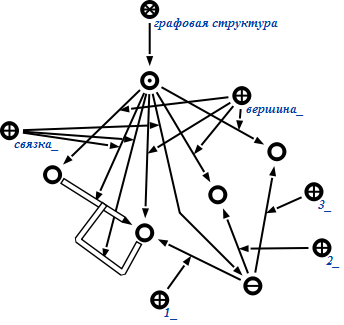
\includegraphics[scale=0.7]{images/1.png}
  \caption{Графовая структура}
\end{figure}

\item
  Графовая структура с ориентированными связками (абсолютное понятие)

  \begin{enumerate}
  \item
    Ориентированная связка (относительное понятие, ролевое отношение)
    -- связка, которая задается ориентированным множеством.
  \end{enumerate}

\begin{figure}[H]
  \centering
  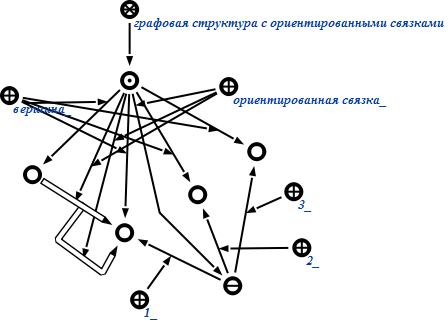
\includegraphics[scale=0.7]{images/2.png}
  \caption{Графовая структура с ориентированными связками}
\end{figure}

\item
  Графовая структура с неориентированными связками (абсолютное понятие)

  \begin{enumerate}
  \item
    Неориентированная связка (относительное понятие, ролевое отношение)
    --связка, которая задается неориентированным множеством.
  \end{enumerate}

\begin{figure}[H]
  \centering
  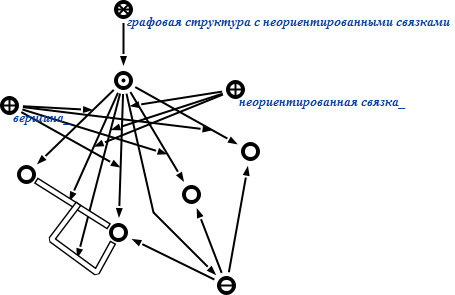
\includegraphics[scale=0.7]{images/3.png}
  \caption{Графовая структура с неориентированными связками}
\end{figure}

\item
  Гиперграф (абсолютное понятие) -- это такая графовая структура, в
  которой связки могут связывать только вершины:

  \begin{enumerate}
  \item
    Гиперсвязка (относительное понятие, ролевое отношение);
  \item
    Гипердуга (относительное понятие, ролевое отношение) --
    ориентированнаягиперсвязка;
  \item
    Гиперребро (относительное понятие, ролевое отношение) --
    неориентированнаягиперсвязка.
  \end{enumerate}

\begin{figure}[H]
  \centering
  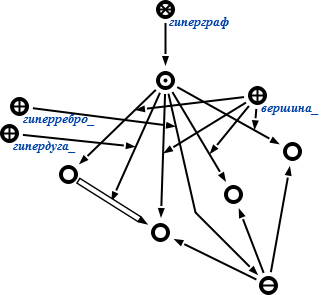
\includegraphics[scale=0.7]{images/4.png}
  \caption{Гиперграф}
\end{figure}

\item
  Псевдограф (абсолютное понятие) -- это такой гиперграф, в котором все
  связки должны быть бинарными:

  \begin{enumerate}
  \item
    Бинарная связка (относительное понятие, ролевое отношение)
    --гиперсвязка арности 2;
  \item
    Ребро (относительное понятие, ролевое отношение)
    --неориентированнаягиперсвязка;
  \item
    Дуга (относительное понятие, ролевое отношение) -- ориентированная
    гиперсвязка;
  \item
    Петля (относительное понятие, ролевое отношение) -- бинарная связка,
    у которой первый и второй компоненты совпадают.
  \end{enumerate}

\begin{figure}[H]
  \centering
  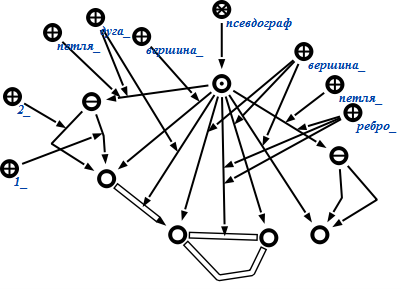
\includegraphics[scale=0.7]{images/5.png}
  \caption{Псевдограф}
\end{figure}

\item
  Мультиграф (абсолютное понятие) -- это такой псевдограф, в котором не
  может быть петель:

\begin{figure}[H]
  \centering
  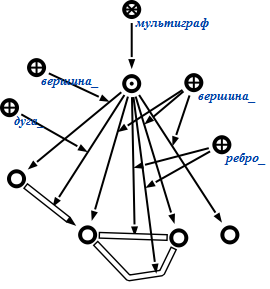
\includegraphics[scale=0.7]{images/6.png}
  \caption{Мультиграф}
\end{figure}

\item
  Граф (абсолютное понятие) -- это такой мультиграф, в котором не может
  быть кратных связок, т.е. связок у которых первый и второй компоненты
  совпадают:

\begin{figure}[H]
  \centering
  \includegraphics[scale=0.7]{images/7.png}
  \caption{Граф}
\end{figure}

\item
  Неориентированный граф (абсолютное понятие) --это такой граф, в
  котором все связки являются ребрами:

\begin{figure}[H]
  \centering
  \includegraphics[scale=0.7]{images/8.png}
  \caption{Неориентированный граф}
\end{figure}

\item
  Ориентированный граф (абсолютное понятие) - это такой граф, в котором
  все связки являются дугами:

\begin{figure}[H]
  \centering
  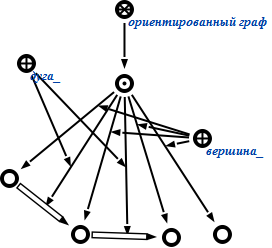
\includegraphics[scale=0.7]{images/9.png}
  \caption{Ориентированный граф}
\end{figure}

\item
  Маршрут (относительное понятие, бинарное ориентированное отношение) --
  это чередующаяся последовательность вершин и гиперсвязок в гиперграфе,
  которая начинается и кончается вершиной, и каждая гиперсвязка
  последовательности инцидентна двум вершинам, одна из которых
  непосредственно предшествует ей, а другая непосредственно следует за
  ней. В примере ниже показан маршрут \emph{A}, \emph{CON1}, \emph{C},
  \emph{CON2}, \emph{D}, \emph{CON3}, \emph{B}, \emph{CON1}, \emph{A} в
  гиперграфе.

\begin{figure}[H]
  \centering
  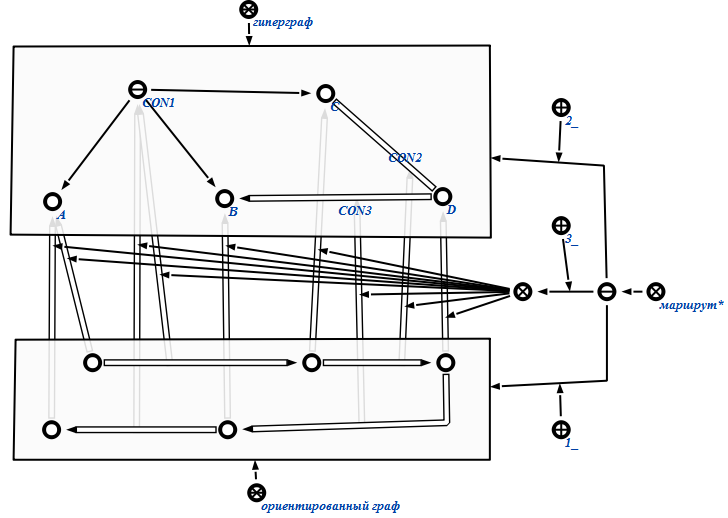
\includegraphics[scale=0.7]{images/10.png}
  \caption{Маршрут}
\end{figure}

\item
  Цепь (относительное понятие, бинарное ориентированное отношение) --
  это маршрут, все гиперсвязки которого различны. В примере ниже
  показана цепь \emph{A}, \emph{CON1}, \emph{C}, \emph{CON2}, \emph{D},
  \emph{CON3}, \emph{B}, \emph{CON4}, \emph{A} в гиперграфе.

\begin{figure}[H]
  \centering
  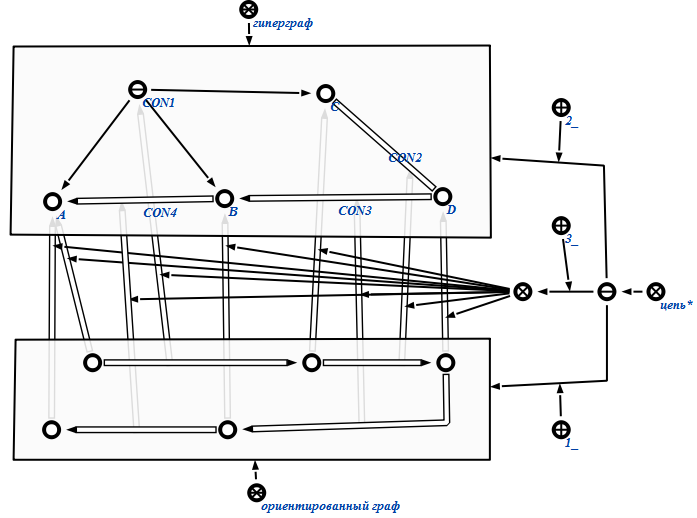
\includegraphics[scale=0.7]{images/11.png}
  \caption{Цепь}
\end{figure}

\item
  Простая цепь, путь (относительное понятие, бинарное ориентированное
  отношение) -- это цепь, в которой все вершины различны. В примере ниже
  показан путь \emph{A}, \emph{CON1}, \emph{C}, \emph{CON2}, \emph{D},
  \emph{CON3}, \emph{B} в гиперграфе.

\begin{figure}[H]
  \centering
  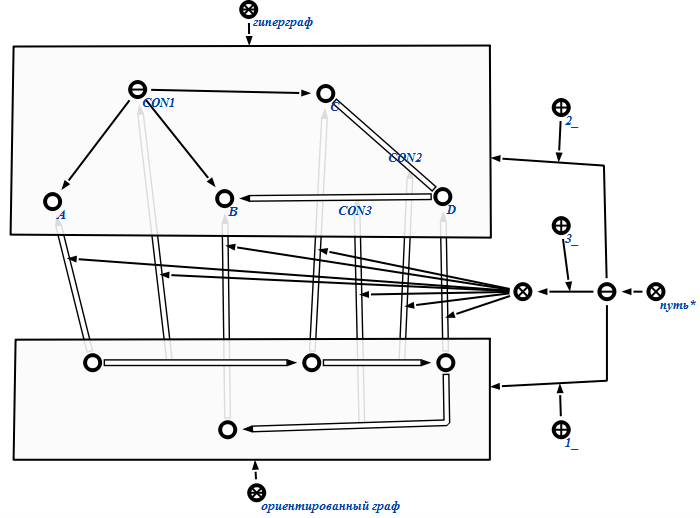
\includegraphics[scale=0.7]{images/12.png}
  \caption{Простая цепь}
\end{figure}

\end{enumerate}

\section{Тестовые примеры}

Во всех тестах графы будет приведены в сокращенной форме со скрытыми ролями элементов графа.

\subsection{Тест 1}

\textbf{Вход:}

Необходимо найти минимальный путь между вершинами A и C.

\begin{figure}[H]
  \centering
  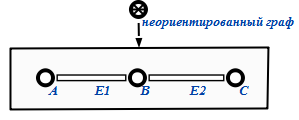
\includegraphics[scale=0.7]{images/13.png}
  \caption{Вход теста 1}
\end{figure}

\textbf{Выход:}

Будет найден единственный минимальный путь \emph{A}, \emph{E1},
\emph{B}, \emph{E2}, \emph{C}:

\begin{figure}[H]
  \centering
  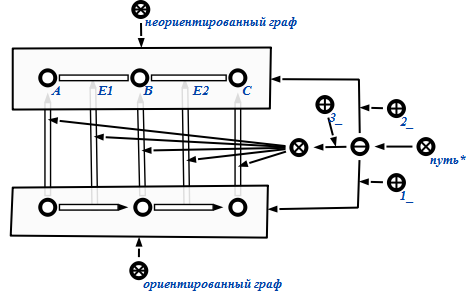
\includegraphics[scale=0.7]{images/14.png}
  \caption{Выход теста 1}
\end{figure}

\subsection{Тест 2}

\textbf{Вход:}

Необходимо найти минимальный путь между вершинами \emph{A} и \emph{F}.

\begin{figure}[H]
  \centering
  \includegraphics[scale=0.7]{images/15.png}
  \caption{Вход теста 2}
\end{figure}

\textbf{Выход:}

Будет найден один из двух минимальный путь \emph{A}, \emph{E2},
\emph{B}, \emph{E3}, \emph{D}, \emph{E5}, \emph{F}:

\begin{figure}[H]
  \centering
  \includegraphics[scale=0.7]{images/16.png}
  \caption{Выход теста 2}
\end{figure}

\subsection{Тест 3}

\textbf{Вход:}

Необходимо найти минимальный путь между вершинами \emph{A} и \emph{K}.

\begin{figure}[H]
  \centering
  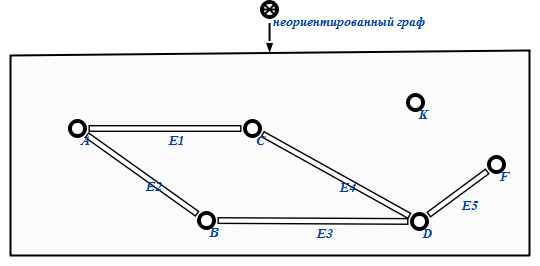
\includegraphics[scale=0.7]{images/17.png}
  \caption{Вход теста 3}
\end{figure}

\textbf{Выход:}

Минимального пути между вершинами \emph{A} и \emph{K} не существует.
Программа должна вернуть ошибку вызывающему контексту.

\subsection{Тест 4}

\textbf{Вход:}

Необходимо найти минимальный путь между вершинами \emph{V5} и
\emph{V11}.

\begin{figure}[H]
  \centering
  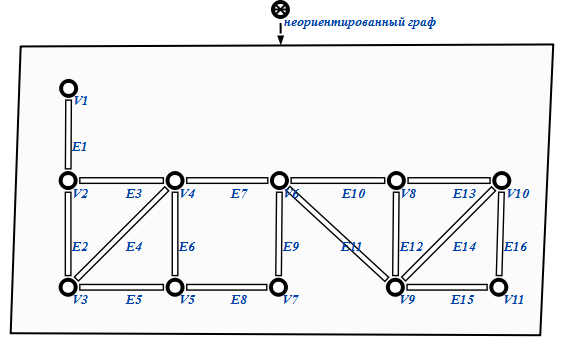
\includegraphics[scale=0.7]{images/18.png}
  \caption{Вход теста 4}
\end{figure}

\textbf{Выход:}

Будет найден один из двух минимальный путь \emph{V5}, \emph{E8},
\emph{V7}, \emph{E9}, \emph{V6}, \emph{E11}, \emph{V9, E15, V11}:

\begin{figure}[H]
  \centering
  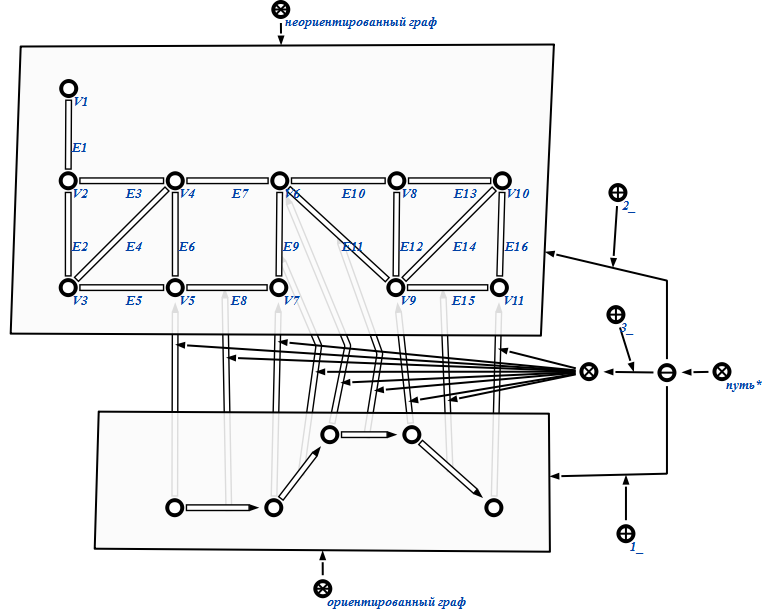
\includegraphics[scale=0.7]{images/19.png}
  \caption{Выход теста 4}
\end{figure}

\subsection{Тест 5}

\textbf{Вход:}

Необходимо найти минимальный путь между вершинами \emph{V1} и \emph{V9}.

\begin{figure}[H]
  \centering
  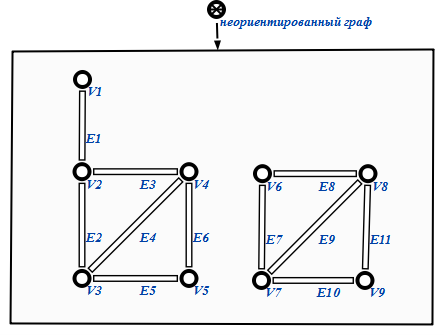
\includegraphics[scale=0.7]{images/20.png}
  \caption{Вход теста 5}
\end{figure}

\textbf{Выход:}

Минимального пути между вершинами \emph{V1} и \emph{V9} не существует. Программа должна вернуть ошибку вызывающему контексту.

\section{Пример работы алгоритма в семантической памяти}

Пример см. в ai\_rr.pdf

% Если в тексте записки есть приложения, для добавления их в содержание, необходимо оставить слудеющую строку
% Если приложений нет - данную строку добавляем в комментарий
\addcontentsline{toc}{section}{Список использованных источников}

\nocite{*}
\selectlanguage{russian}
\bibliography{bibliography}


\end{document}
